\chapter{Methodology}
\label{chapter:methodology}

We have shown that reservoir computing using Random Boolean Networks is a feasible approach to solving binary time-series problems.
We now wish to investigate which parameters and characteristics of the reservoir lead to optimal performance and resource usage.

The following questions arise:

\begin{enumerate}
    \item How small can a RBN Reservoir System be while still solving a given task at close to 100\% accuracy?
    \item How many connections from the input layer are required to sufficiently perturb the reservoir?
    \item How few reservoir nodes can be connected to the readout layer while maintaining task accuracy?
    \item Is there a correlation between the dynamical characteristics of the RBN (number of attractors, attractor length) and its performance as a reservoir?
\end{enumerate}

The answers to these questions aren't 'just' of theoretical interest,
they also give us insight to how physical reservoir computing devices have to be instrumented.

In a physical substrate it might be prohibitively expensive or technologically infeasible to read the state of the entire reservoir,
and the nodes you are able to measure might be affected by the 'values' of the nodes next to it.
In the case of a growing and modifying reservoir, such as a stem-cell based reservoir,
the topology of the network might change over time without having the ability to reinstrument the device.
A finding that it's enough to use a subset of the available nodes for regression in the readout layer,
regardless of reservoir size, would be of practical interest.

There are two factors affecting optimal reservoir perturbance:
There might be a problem-specific optimal perturbance dependent on the task at hand as well as connectivity of the reservoir and number of runs after each perturbance.
For physical devices one is in addition limited by the physical characteristics of the reservoir,
such as cost and the number of available electrodes for instrumenting limited by physical space.

Finding the minimum required size of a RBN Reservoir for a given task allows us to create physical reservoirs with adequate computational abilities guided by the theoretical foundations described herein ("Helmax setning, Egon! Helmax!").

Finally, we attempt to explain the performance of RBN Reservoirs through their dynamical properties,
calculating the number of attractors and their length for reservoirs against their accuracy on a given task.
A correlation between these properties might be interesting, and help to explain why some reservoirs perform better than others.

\section{Experimental setup}

The final RRC system is shown as a block diagram in Figure \ref{figure:rrc-block},
and the actual network topology is equivalent to the one in Figure \ref{figure:rbn-reservoir}.

\todo{so much todo}
\todo{Explain every box line in the box diagram, probably with more stuff}

\todo{gotta add moar stuffz here, nemlig varierende input/output cocnnectivitet støtte}

\begin{figure}
    \centering
    \begin{tikzpicture}
        \node (dataset) {Dataset};
        \node[box, below=of dataset] (input) {Input layer};
        \node[box, right=of input] (reservoir) {RBN Reservoir};
        \node[box, right=of reservoir] (readout) {Readout layer};
        \node[above=of readout] (classification) {Classification};

        \node[draw,dotted,fit=(input) (reservoir) (readout), label={RRC}] {};

        \draw[edge] (dataset) to (input);
        \draw[edge] (input) to (reservoir);
        \draw[edge] (reservoir) to (readout);
        \draw[edge] (readout) to (classification);
    \end{tikzpicture}
    \caption{Block diagram of the RRC processing a dataset.}
    \label{figure:rrc-block}
\end{figure}

\subsection{testing}

To verify that RBN simulation is working,
a RBN is created randomly, initial state set to all zeros, and ran.
The results are visualized in Figure \ref{figure:rbn-noperturb}.
We see that the RBN exhibits stable dynamics, and enters into an attractor around $t=15$.
In Figure \ref{figure:rbn-perturb} we continiously perturb the RBN with the input stream from the Temporal Parity task visualized in Figure \ref{figure:temporal-parity}.
In the perturbed case, the state trajectory is continiously changed, preventing the RBN from settling into an attractor.
Interestingly enough, there seems to be a visual similarity between the two cases.
Such a pattern is sure to dissapear with a RBN in the chaotic phase.

This erratic pattern of state transitions is then fed into the readout layer,
which is then tasked with finding a linear combination of the RBN states that results in the expected output for the given task.

\begin{figure}
  \subfloat[Unperturbed]{
    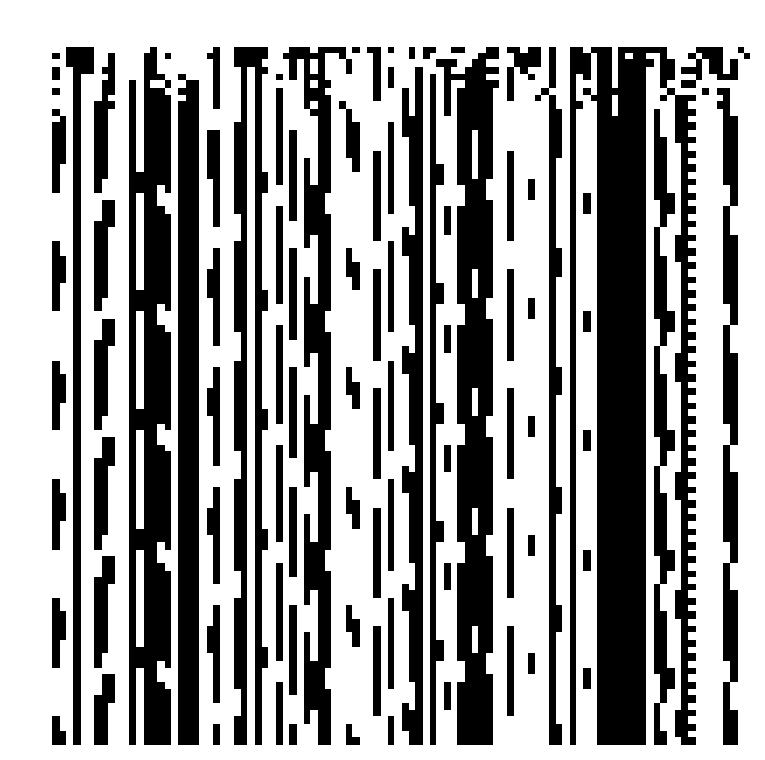
\includegraphics[width=0.5\columnwidth]{method/final-1-noperturb.pdf}
    \label{figure:rbn-noperturb}
  }
  \subfloat[Perturbed]{
    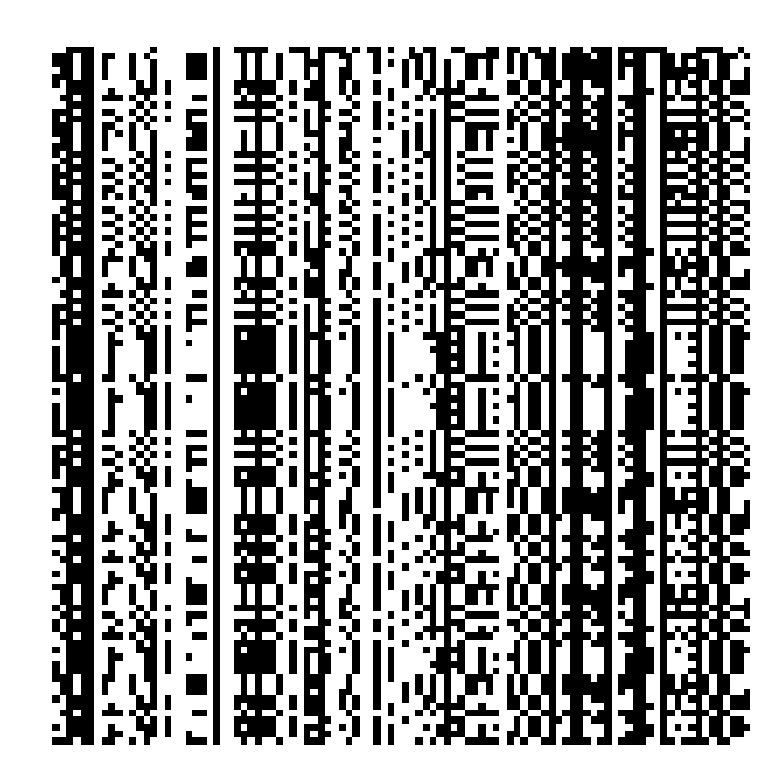
\includegraphics[width=0.5\columnwidth]{method/final-1-perturb.pdf}
    \label{figure:rbn-perturb}
  }
  \caption{
    The same RBN ($N=100, K=2, P=0.5, L=50$) shown both perturbed and unperturbed.
    The boolean states of the RBN are plotted along the X-axis,
    with time flowing downwards.
  }
\end{figure}

\subsection{Training}

To train the RRC system we require large training datasets,
as well as different, smaller datasets for testing the trained system.
We will use the datasets described in section \ref{subsection:rbn-reservoir-systems}.

We then either create a new RBN (initialize it randomly),
or load a previously created RBN from disk.
For each bit of input in each dataset,
we perturb the input-connected nodes in the RBN.
After each perturbance, the RBN is ran synchronously (CRBN mode) for one timestep.
The resulting RBN states are collected,
and after the entire dataset is processed,
forwarded to the readout layer.

To find a suitable mapping from the set of reservoir states and the correct input classification,
ridge regression \cite{hoerl1970ridge} is used.
This version of least squares regression is more accurate when faced with input colinearities, as well as always being at least as accurate as ordinary least squares.  
This process is repeated for all the datasets,
and the final regression parameters are chosen as a combination of the parameters obtained for each individual dataset.
Finally we measure the normalized accuracy of the trained reservoir on the test dataset,
defined as the following:
\begin{equation}
Accuracy = 1 - \dfrac{sum(actual\_output \neq expected\_output)}{len(correct\_output)}
\label{formula:accuracy}
\end{equation}
